\documentclass[journal,letterpaper]{IEEEtran}
\usepackage[utf8]{inputenc}
\usepackage[spanish]{babel}
\usepackage{amsmath}
\usepackage{graphicx}
\usepackage{booktabs}
\usepackage{hyperref}
\usepackage{microtype}
\usepackage{array}
\usepackage{multirow}
\graphicspath{{figures/}}

\begin{document}

\title{Reporte de Sprint 3: Hiperparametrización, Selección del Modelo Final y Exportación del Clasificador de Clientes Premium}

\author{Marcelo de la Quintana,
        Gaston Nina,
        y~Gerick Toro\\
        \textit{Módulo de Implementación de Soluciones de Inteligencia Artificial}\\
        \textit{Maestría en Inteligencia Artificial y Ciencia de Datos}}

\markboth{INFORME TÉCNICO - SPRINT 3, JUNIO 2026}%
{Sprint 3: Hiperparametrización y Modelo Final de Clientes Premium}

\maketitle

\begin{abstract}
Este informe documenta el Sprint 3 del proyecto analítico sobre la plataforma Olist, cuyo objetivo fue seleccionar el algoritmo de clasificación de clientes premium con mayor capacidad predictiva y optimizar sus hiperparámetros para producir el artefacto de modelo serializado listo para producción. Partiendo de las 28 variables del experimento \texttt{corr\_le\_0.85} del Sprint 2 y del mismo split temporal (\textit{train}: \texttt{last\_purchase} $<$ 2018-07-01; \textit{validación}: $\geq$ 2018-07-01), se evaluaron cinco modelos candidatos en configuración base: Regresión Logística, Random Forest, Gradient Boosting, XGBoost y LightGBM. El benchmark inicial confirmó a LightGBM (ROC-AUC$_{\text{val}}$ = 0.8035, Gini$_{\text{val}}$ = 0.6070) y XGBoost (ROC-AUC$_{\text{val}}$ = 0.7982, Recall$_{\text{val}}$ = 0.6906) como modelos finalistas mediante un ranking compuesto que pondera capacidad discriminante y cobertura del segmento premium. La optimización de hiperparámetros con \textbf{Optuna TPE} (50 \textit{trials} por modelo) mejoró el ROC-AUC de LightGBM a \textbf{0.8081} (+0.0046) y el de XGBoost a 0.8070 (+0.0088). LightGBM se consolidó como modelo ganador por liderar en todas las métricas de discriminación global, con un gap de sobreajuste controlado de 0.039. El umbral óptimo de decisión (0.55) maximiza el F1-Score a 0.5603. Las variables \texttt{top\_category} y \texttt{recency\_days} concentran el 43\% de la importancia de ganancia del modelo. El pipeline serializado (\texttt{modelo\_final.pkl}) supera en 1.52 puntos de ROC-AUC y 3.23 puntos de Recall al Random Forest del Sprint 2, estableciendo la base técnica para el despliegue en el Sprint 4.
\end{abstract}

\begin{IEEEkeywords}
LightGBM, XGBoost, Optuna, Hiperparametrización, Clasificación Supervisada, Clientes Premium, Olist, ROC-AUC, Gini, Feature Importance.
\end{IEEEkeywords}

% ──────────────────────────────────────────────────────────────────
\section{Introducción}
\IEEEPARstart{E}{l} Sprint 2 entregó un pipeline reproducible de ingeniería de variables que elevó el ROC-AUC de clasificación de clientes premium de 0.5355 (baseline logístico del Sprint 1) a \textbf{0.7929} usando un Random Forest con 28 features del experimento \texttt{corr\_le\_0.85}~\cite{sprint2_report}. Esa mejora confirmó que la \textbf{Paradoja del Target}~\cite{sprint1_report} —donde el 97\% de los clientes de Olist tiene una única orden— puede ser abordada con variables de comportamiento de categoría de producto, logística y método de pago, más allá del esquema RFMT tradicional~\cite{rfmt_methodology}.

El \textbf{Sprint 3} tiene como objetivo responder: \textit{¿qué algoritmo y con qué configuración de hiperparámetros maximiza la capacidad de identificar clientes premium sobre las 28 variables validadas?} Para ello se diseñó un flujo de cuatro etapas:

\begin{enumerate}
    \item \textbf{S3-DS-01}: Benchmark inicial de cinco modelos candidatos en configuración base, con el mismo split temporal y features del Sprint 2.
    \item \textbf{S3-DS-02}: Selección de modelos finalistas mediante criterio compuesto de métricas técnicas y contexto de negocio.
    \item \textbf{S3-DS-03/04}: Optimización de hiperparámetros (HPO) de los finalistas con Optuna TPE, 50 \textit{trials} por modelo.
    \item \textbf{Evaluación y exportación}: Verificación de reproducibilidad del pipeline serializado.
\end{enumerate}

La motivación de negocio permanece intacta desde el Sprint 1: el segmento premium (20\% de los clientes) concentra el \textbf{56.03\%} de la facturación de Olist, con un ticket promedio \textbf{4.36 veces} superior al del cliente regular (BRL 402.66 vs. BRL 92.27)~\cite{sprint2_report}. En este contexto, \textbf{Recall es la métrica de negocio prioritaria}: un falso negativo implica perder la oportunidad de retención sobre el segmento de mayor valor.

% ──────────────────────────────────────────────────────────────────
\section{Configuración Experimental}

\subsection{Datos y Split Temporal}
Se utilizó el dataset oficial de features del Sprint 2 (\texttt{06\_features\_selected.parquet}), con 96.096 clientes y 28 variables. Para aplicar el split temporal fue necesario combinar este archivo con \texttt{05\_features\_rfm.parquet} (fuente de \texttt{last\_purchase}), ya que dicha columna fue excluida del set de features por ser información temporal que no estaría disponible en producción.

\begin{table}[h]
\centering
\caption{Partición de Datos — Sprint 3}
\label{tab:split}
\begin{tabular}{lrr}
\toprule
Conjunto & Criterio & Registros \\
\midrule
Train & \texttt{last\_purchase} $<$ 2018-07-01 & 83.589 \\
Validación & \texttt{last\_purchase} $\geq$ 2018-07-01 & 6.230 \\
\midrule
\multicolumn{2}{l}{Tasa premium en train} & 21.29\% \\
\multicolumn{2}{l}{Tasa premium en validación} & 22.83\% \\
\bottomrule
\end{tabular}
\end{table}

\subsection{Preprocesamiento}
Todos los modelos comparten el mismo preprocesador encapsulado en un \texttt{ColumnTransformer} de scikit-learn:
\begin{itemize}
    \item \textbf{Variables numéricas (22):} imputación por mediana (\texttt{SimpleImputer}).
    \item \textbf{Variables categóricas (6):} imputación por moda + codificación \texttt{OneHotEncoder} con \texttt{handle\_unknown='ignore'}.
\end{itemize}

El preprocesador se ajusta (\textit{fit}) exclusivamente sobre el conjunto de train y se aplica (\textit{transform}) sobre validación, garantizando la ausencia de fuga de información en la normalización.

\subsection{Desbalance de Clases}
La proporción de clientes regulares frente a premium en train es aproximadamente 3.70:1. Para compensar este desbalance sin submuestreo (lo que preserva toda la información de entrenamiento), cada modelo recibe la corrección apropiada:
\begin{itemize}
    \item \texttt{class\_weight='balanced'}: Regresión Logística, LightGBM.
    \item \texttt{class\_weight='balanced\_subsample'}: Random Forest.
    \item \texttt{scale\_pos\_weight=3.70}: XGBoost.
    \item Sin ajuste explícito: Gradient Boosting (sklearn), que por diseño es menos sensible al desbalance en su implementación interna.
\end{itemize}

% ──────────────────────────────────────────────────────────────────
\section{S3-DS-01: Benchmark de Modelos Candidatos}

\subsection{Modelos Evaluados}
La Tabla~\ref{tab:models} describe los cinco modelos candidatos con su configuración base.

\begin{table}[h]
\centering
\caption{Modelos Candidatos — Configuración Base}
\label{tab:models}
\resizebox{\columnwidth}{!}{%
\begin{tabular}{lll}
\toprule
Modelo & Tipo & Configuración base \\
\midrule
\texttt{logistic\_regression} & Lineal & \texttt{class\_weight='balanced'}, scaler \\
\texttt{random\_forest}       & Bagging & 200 árboles, \texttt{balanced\_subsample} \\
\texttt{gradient\_boosting}   & Boosting sklearn & 200 estimadores, \texttt{lr}=0.05 \\
\texttt{xgboost}              & Boosting XGB & 250 estim., \texttt{scale\_pos\_weight}=3.70 \\
\texttt{lightgbm}             & Boosting LGBM & 250 estim., \texttt{class\_weight='balanced'} \\
\bottomrule
\end{tabular}%
}
\end{table}

\subsection{Resultados del Benchmark}
La Tabla~\ref{tab:benchmark} presenta las métricas de validación de los cinco modelos, ordenadas por ROC-AUC descendente. La columna \textit{Gap} representa la diferencia entre ROC-AUC en train y en validación, como indicador de sobreajuste.

\begin{table}[h]
\centering
\caption{Benchmark Inicial — Métricas en Validación}
\label{tab:benchmark}
\resizebox{\columnwidth}{!}{%
\begin{tabular}{lrrrrrr}
\toprule
Modelo & AUC val & Gini val & PR-AUC & F1 val & Recall val & Gap \\
\midrule
\textbf{lightgbm}        & \textbf{0.8035} & \textbf{0.6070} & 0.5954 & \textbf{0.5565} & 0.6653 & 0.037 \\
gradient\_boosting        & 0.7985 & 0.5970 & 0.5881 & 0.4524 & 0.3340 & 0.027 \\
xgboost                   & 0.7982 & 0.5964 & 0.5896 & 0.5504 & \textbf{0.6906} & 0.029 \\
random\_forest             & 0.7926 & 0.5852 & 0.5677 & 0.5422 & 0.6392 & 0.019 \\
logistic\_regression       & 0.7884 & 0.5768 & 0.5661 & 0.5329 & 0.6456 & 0.016 \\
\bottomrule
\end{tabular}%
}
\end{table}

La Figura~\ref{fig:benchmark_auc} ilustra visualmente la comparación entre ROC-AUC de train y validación para los cinco modelos.

\begin{figure}[h]
  \centering
  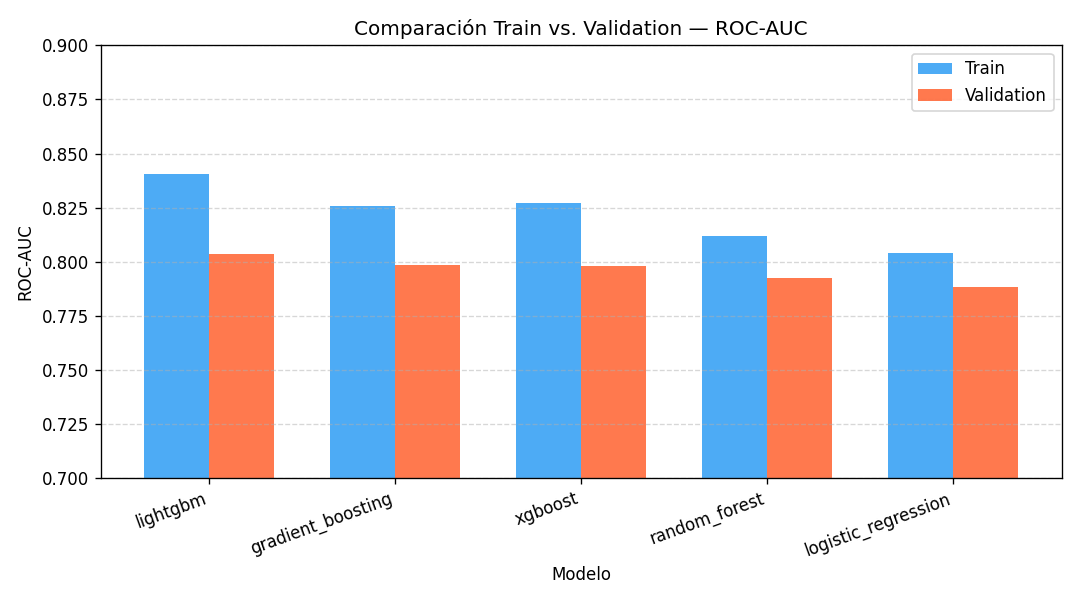
\includegraphics[width=\columnwidth]{fig_benchmark_auc.png}
  \caption{Comparación de ROC-AUC train vs. validación para los cinco modelos candidatos. El gap moderado de LightGBM (0.037) y XGBoost (0.029) es aceptable para la fase de tuning.}
  \label{fig:benchmark_auc}
\end{figure}

\subsection{Continuidad con el Sprint 2}
El resultado de \texttt{random\_forest} en validación (ROC-AUC = 0.7926) es prácticamente idéntico al resultado oficial del Sprint 2 (\texttt{corr\_le\_0.85}, ROC-AUC = 0.7929). Esta diferencia de 0.0003 confirma la reproducibilidad del pipeline y que el benchmark parte de una base estable.

Los modelos de boosting mejoran el baseline del Sprint 2 entre +0.6 y +1.1 puntos de ROC-AUC, validando la hipótesis de que algoritmos de mayor capacidad no lineal capturan mejor los patrones de la Paradoja del Target.

% ──────────────────────────────────────────────────────────────────
\section{S3-DS-02: Selección de Modelos Finalistas}

\subsection{Criterios de Selección}
La selección de finalistas aplicó cuatro criterios combinados. Los umbrales mínimos de AUC y Gini garantizan mejora real sobre el Sprint 2; el límite de gap controla el riesgo de sobreajuste en producción.

\begin{table}[h]
\centering
\caption{Criterios de Selección de Finalistas}
\label{tab:criteria}
\begin{tabular}{lll}
\toprule
Criterio & Umbral & Justificación \\
\midrule
ROC-AUC val & $\geq 0.78$ & Mejora sobre baseline S2 \\
Gini val & $\geq 0.56$ & Equivalente a AUC $\geq 0.78$ \\
Gap overfit & $\leq 0.06$ & Estabilidad aceptable \\
Ranking compuesto & Top 2 & $0.5 \times \text{AUC} + 0.3 \times \text{Gini} + 0.2 \times \text{F1}$ \\
\bottomrule
\end{tabular}
\end{table}

El ranking compuesto incorpora F1 para penalizar modelos con Recall bajo. Esta decisión fue determinante: \texttt{gradient\_boosting} supera a XGBoost en ROC-AUC por 0.0003 (0.7985 vs. 0.7982), pero su Recall de \textbf{0.33} significaría dejar sin detectar al 67\% de los clientes premium, perdiendo el acceso al segmento responsable del 56\% de la facturación. El ranking compuesto selecciona correctamente a XGBoost sobre Gradient Boosting gracias al componente F1 (0.5504 vs. 0.4524).

\subsection{Finalistas Seleccionados}
Los modelos finalistas son \textbf{LightGBM} y \textbf{XGBoost}, con los argumentos técnicos resumidos en la Tabla~\ref{tab:finalists}.

\begin{table}[h]
\centering
\caption{Argumentos Técnicos por Finalista}
\label{tab:finalists}
\resizebox{\columnwidth}{!}{%
\begin{tabular}{lrr}
\toprule
Argumento & LightGBM & XGBoost \\
\midrule
ROC-AUC val     & \textbf{0.8035} & 0.7982 \\
Gini val        & \textbf{0.6070} & 0.5964 \\
Recall val      & 0.6653 & \textbf{0.6906} \\
F1 val          & \textbf{0.5565} & 0.5504 \\
Gap overfit     & 0.037 & \textbf{0.029} \\
Fortaleza       & Discriminación global & Mayor Recall base \\
\bottomrule
\end{tabular}%
}
\end{table}

% ──────────────────────────────────────────────────────────────────
\section{S3-DS-03/04: Optimización de Hiperparámetros}

\subsection{Metodología: Optuna TPE}
La optimización de hiperparámetros (HPO) se realizó con \textbf{Optuna}~\cite{optuna2019} usando el método de muestreo \textbf{TPE} (Tree-structured Parzen Estimator). A diferencia de la búsqueda por grilla (GridSearchCV), TPE construye un modelo probabilístico del espacio de hiperparámetros basado en los \textit{trials} anteriores, dirigiendo la búsqueda hacia las regiones con mayor probabilidad de mejora. Esta estrategia bayesiana es significativamente más eficiente que GridSearch en espacios continuos de alta dimensión~\cite{bergstra2011}.

\textbf{Configuración:} 50 \textit{trials} por modelo; objetivo de maximización: ROC-AUC en validación; semilla fija para reproducibilidad (\texttt{seed=42}).

\subsection{Espacio de Búsqueda — LightGBM}
La Tabla~\ref{tab:lgbm_space} resume el espacio de hiperparámetros explorado para LightGBM.

\begin{table}[h]
\centering
\caption{Espacio de Búsqueda HPO — LightGBM}
\label{tab:lgbm_space}
\resizebox{\columnwidth}{!}{%
\begin{tabular}{lll}
\toprule
Hiperparámetro & Rango & Escala \\
\midrule
\texttt{num\_leaves}        & [20, 150]   & Entero \\
\texttt{max\_depth}         & [3, 10]     & Entero \\
\texttt{learning\_rate}     & [0.01, 0.20] & Log-uniforme \\
\texttt{n\_estimators}      & [100, 500]  & Entero \\
\texttt{min\_child\_samples} & [10, 100]   & Entero \\
\texttt{subsample}          & [0.6, 1.0]  & Uniforme \\
\texttt{colsample\_bytree}  & [0.6, 1.0]  & Uniforme \\
\texttt{reg\_alpha}         & [$10^{-8}$, 1.0] & Log-uniforme \\
\texttt{reg\_lambda}        & [$10^{-8}$, 1.0] & Log-uniforme \\
\bottomrule
\end{tabular}%
}
\end{table}

XGBoost exploró un espacio equivalente con sus parámetros nativos (\texttt{max\_depth}, \texttt{min\_child\_weight}, \texttt{gamma}, \texttt{reg\_alpha}, \texttt{reg\_lambda}).

La Figura~\ref{fig:optuna_history} muestra la evolución del ROC-AUC a lo largo de los 50 \textit{trials} para cada modelo, donde se aprecia la convergencia progresiva del mejor valor acumulado.

\begin{figure}[h]
  \centering
  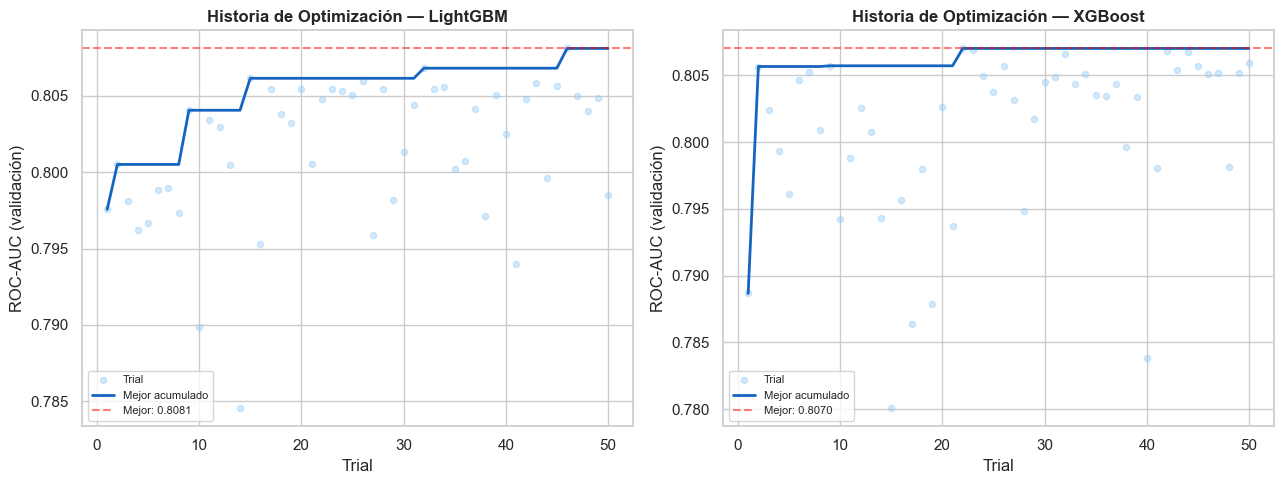
\includegraphics[width=\columnwidth]{fig_optuna_history.png}
  \caption{Historia de optimización Optuna TPE (50 \textit{trials} por modelo). Cada punto representa un \textit{trial} individual; la línea continua muestra el mejor valor acumulado. Ambos modelos convergen tras aproximadamente 30 \textit{trials}.}
  \label{fig:optuna_history}
\end{figure}

\subsection{Hiperparámetros Óptimos — LightGBM (Ganador)}
\begin{equation}
\boldsymbol{\theta}^* = \{n_l{=}59,\; d{=}8,\; \eta{=}0.054,\; T{=}255,\; m{=}68,\; s{=}0.906,\; c{=}0.855\}
\end{equation}
donde $n_l$ = \texttt{num\_leaves}, $d$ = \texttt{max\_depth}, $\eta$ = \texttt{learning\_rate}, $T$ = \texttt{n\_estimators}, $m$ = \texttt{min\_child\_samples}, $s$ = \texttt{subsample}, $c$ = \texttt{colsample\_bytree}.

\subsection{Resultados del Tuning}
La Tabla~\ref{tab:tuning} compara las métricas baseline y post-tuning de ambos finalistas.

\begin{table}[h]
\centering
\caption{Resultados de HPO: Baseline vs. Tuneado}
\label{tab:tuning}
\resizebox{\columnwidth}{!}{%
\begin{tabular}{lrrrrrr}
\toprule
Modelo & AUC val & Gini val & PR-AUC & F1 val & Recall val & Gap \\
\midrule
LGBM baseline   & 0.8035 & 0.6070 & 0.5954 & 0.5565 & 0.6653 & 0.037 \\
\textbf{LGBM tuneado} & \textbf{0.8081} & \textbf{0.6162} & \textbf{0.6010} & \textbf{0.5576} & 0.6617 & 0.039 \\
XGB baseline    & 0.7982 & 0.5964 & 0.5896 & 0.5504 & \textbf{0.6906} & 0.029 \\
XGB tuneado     & 0.8070 & 0.6140 & 0.5997 & 0.5560 & 0.6505 & 0.054 \\
\bottomrule
\end{tabular}%
}
\end{table}

La Figura~\ref{fig:tuning_comparison} ilustra el delta de mejora entre baseline y tuneado para las tres métricas principales.

\begin{figure}[h]
  \centering
  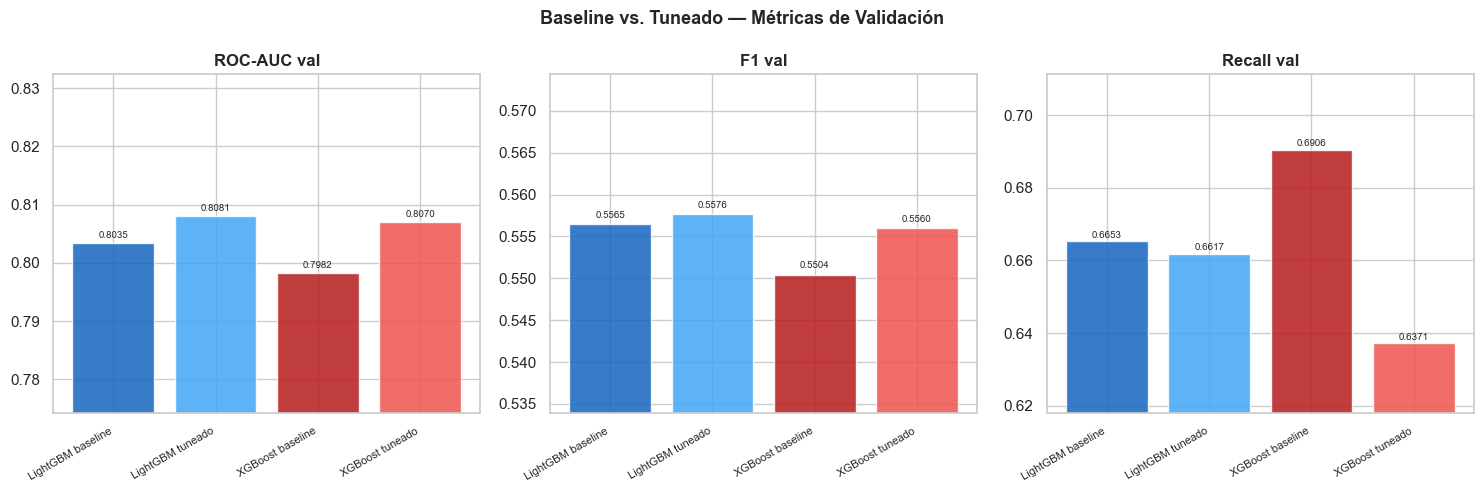
\includegraphics[width=\columnwidth]{fig_tuning_comparison.png}
  \caption{Comparación de métricas baseline vs. tuneado para LightGBM y XGBoost. El tuning de XGBoost logra la mayor ganancia en ROC-AUC (+0.0088), pero a costa de reducir el Recall de 0.6906 a 0.6505.}
  \label{fig:tuning_comparison}
\end{figure}

\textbf{Observación sobre XGBoost tuneado:} La optimización elevó el ROC-AUC de XGBoost en +0.0088, la mayor ganancia absoluta entre ambos modelos. Sin embargo, el Recall descendió de 0.6906 a 0.6505, ya que Optuna maximizó ROC-AUC y no Recall directamente. Si el objetivo de negocio fuera maximizar la cobertura del segmento premium, una corrida adicional de HPO con Recall como función objetivo podría revertir este trade-off. Para el presente sprint, la selección del ganador prioriza las métricas de discriminación global.

% ──────────────────────────────────────────────────────────────────
\section{Modelo Final: LightGBM Tuneado}

\subsection{Justificación de la Selección}
LightGBM tuneado es seleccionado como modelo de producción por cuatro razones:
\begin{enumerate}
    \item \textbf{Mayor ROC-AUC y Gini}: 0.8081 y 0.6162, liderando en discriminación global.
    \item \textbf{Gap de sobreajuste controlado}: 0.039, inferior al umbral crítico de 0.06 definido en los criterios de selección.
    \item \textbf{Velocidad de entrenamiento}: LightGBM es significativamente más rápido que XGBoost en datasets de más de 50.000 filas, lo que facilita las iteraciones de reentrenamiento mensual del Sprint 4.
    \item \textbf{Feature importance nativa}: la ganancia por característica es directamente interpretable y comparable entre modelos, facilitando la comunicación con el equipo de negocio.
\end{enumerate}

\subsection{Métricas en Validación}
La Tabla~\ref{tab:final_metrics} presenta las métricas del modelo final bajo dos umbrales de decisión.

\begin{table}[h]
\centering
\caption{Métricas del Modelo Final — LightGBM Tuneado}
\label{tab:final_metrics}
\begin{tabular}{lrr}
\toprule
Métrica & Umbral 0.50 & Umbral 0.55 \\
\midrule
ROC-AUC   & \multicolumn{2}{c}{0.8081} \\
Gini      & \multicolumn{2}{c}{0.6162} \\
PR-AUC    & \multicolumn{2}{c}{0.6010} \\
\midrule
Precision  & 0.4818 & 0.5225 \\
Recall     & 0.6617 & 0.6041 \\
F1-Score   & 0.5576 & \textbf{0.5603} \\
\midrule
Gap overfit & \multicolumn{2}{c}{0.039} \\
\bottomrule
\end{tabular}
\end{table}

\subsection{Análisis del Umbral de Decisión}
El umbral de decisión controla el trade-off entre Precision y Recall. El umbral por defecto de scikit-learn es 0.50, pero el umbral que maximiza el F1-Score sobre el conjunto de validación es \textbf{0.55}, que reduce levemente el Recall (+0.6617 $\to$ 0.6041) a cambio de elevar la Precision (0.4818 $\to$ 0.5225), mejorando el F1 en 0.0027 puntos.

La Figura~\ref{fig:threshold} ilustra la evolución de las tres métricas en función del umbral de clasificación.

\begin{figure}[h]
  \centering
  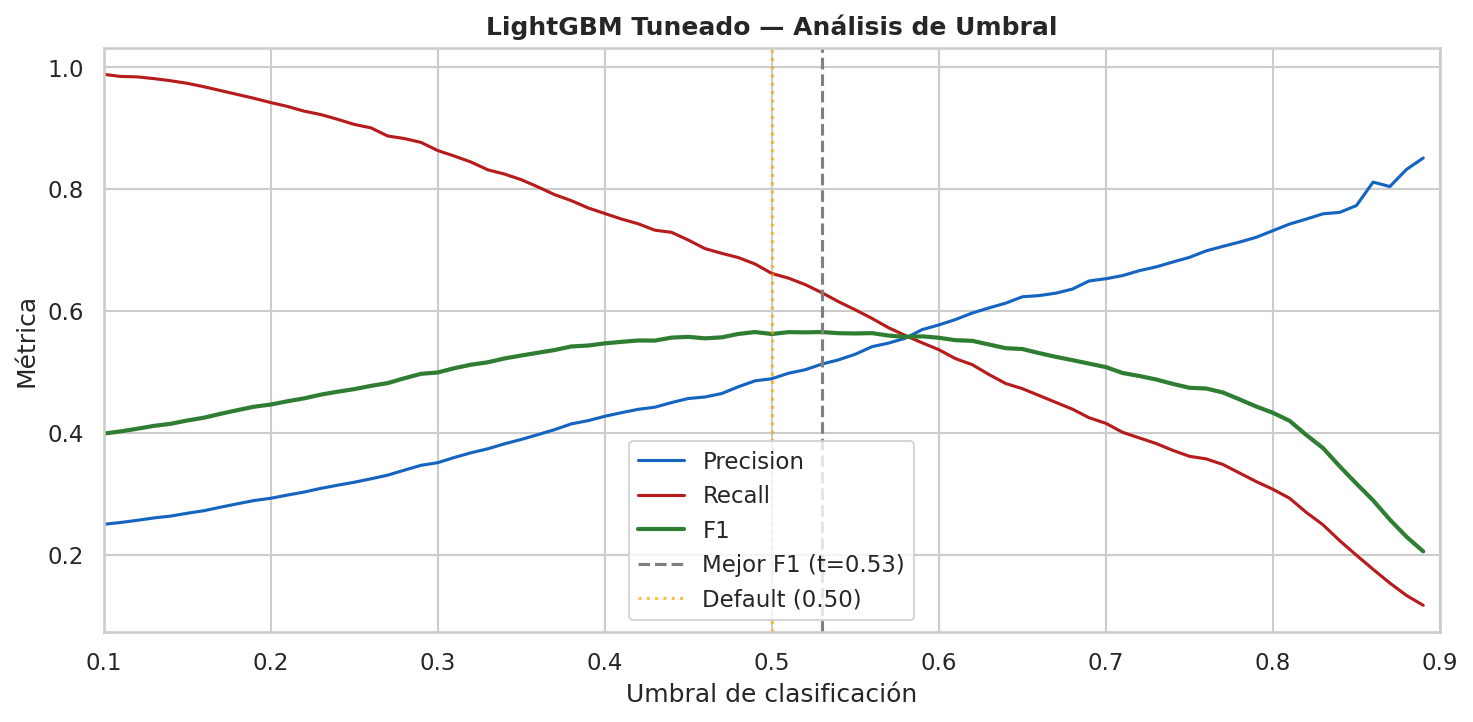
\includegraphics[width=\columnwidth]{fig_threshold_analysis.png}
  \caption{Evolución de Precision, Recall y F1 en función del umbral de decisión. El umbral óptimo (0.55, línea discontinua gris) maximiza el F1-Score. El umbral por defecto (0.50, línea naranja punteada) favorece el Recall.}
  \label{fig:threshold}
\end{figure}

La elección final del umbral de producción es una decisión de negocio. Para el Sprint 4, se recomienda:
\begin{itemize}
    \item \textbf{Umbral 0.50}: si la prioridad es maximizar la cobertura del segmento premium (Recall = 0.66).
    \item \textbf{Umbral 0.55}: si se busca el mejor equilibrio F1 (Recall = 0.60, Precision = 0.52).
\end{itemize}

\subsection{Matriz de Confusión}
Sobre los 6.230 clientes de validación (1.422 premium reales), la Tabla~\ref{tab:confusion} presenta la matriz de confusión con el umbral óptimo 0.55.

\begin{table}[h]
\centering
\caption{Matriz de Confusión — LightGBM Tuneado (umbral = 0.55)}
\label{tab:confusion}
\begin{tabular}{llrr}
\toprule
 & & \multicolumn{2}{c}{Predicción} \\
 & & Regular (0) & Premium (1) \\
\midrule
\multirow{2}{*}{Real} & Regular (0) & TN = 4.023 & FP = 785 \\
                       & Premium (1) & FN = 563   & TP = 859 \\
\bottomrule
\end{tabular}
\end{table}

El modelo detecta correctamente a \textbf{859 de 1.422 clientes premium} (Recall = 60.4\%). Los 563 falsos negativos representan clientes de alto valor no identificados; los 785 falsos positivos son clientes regulares clasificados erróneamente como premium.

La Figura~\ref{fig:confusion} compara las matrices bajo ambos umbrales.

\begin{figure}[h]
  \centering
  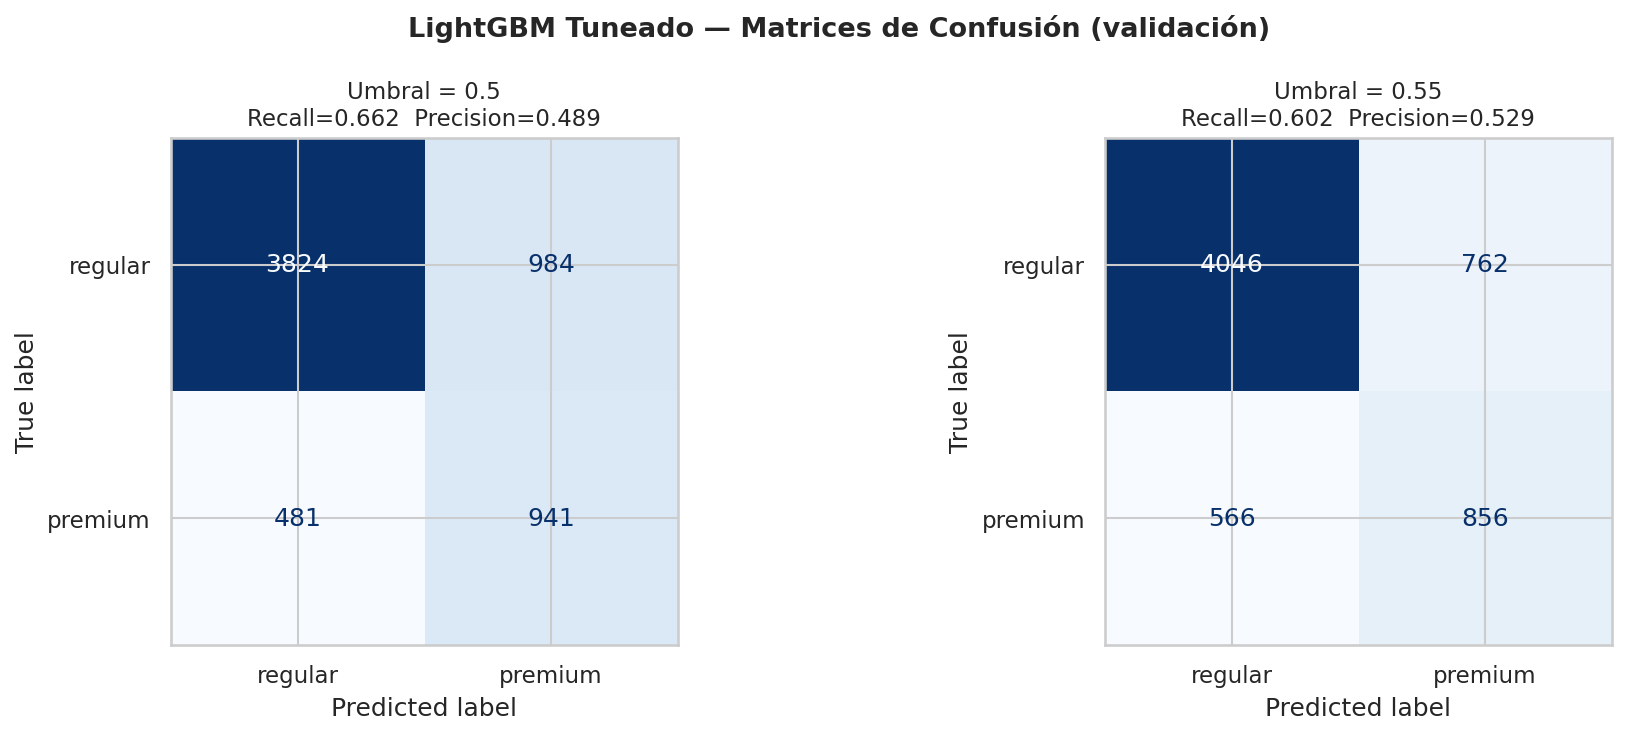
\includegraphics[width=\columnwidth]{fig_confusion_matrix.png}
  \caption{Matrices de confusión del modelo final para los umbrales 0.50 (izquierda) y 0.55 (derecha). El umbral 0.55 reduce los falsos positivos a cambio de un leve aumento en los falsos negativos.}
  \label{fig:confusion}
\end{figure}

\subsection{Curvas ROC y Precision-Recall}
La Figura~\ref{fig:roc_pr} presenta las curvas ROC y Precision-Recall del modelo final junto a las referencias de clasificación aleatoria.

\begin{figure}[h]
  \centering
  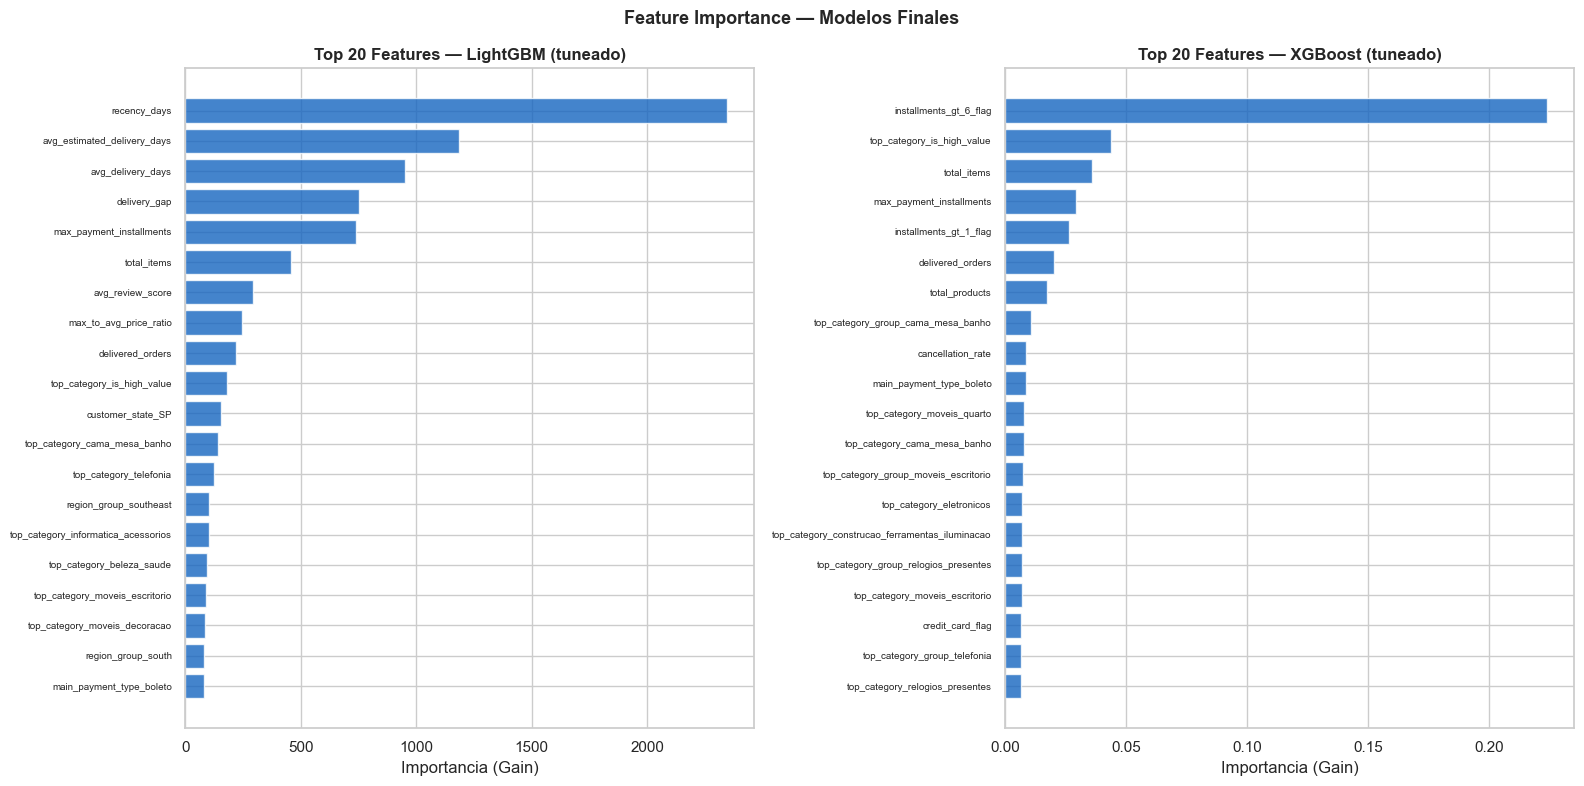
\includegraphics[width=\columnwidth]{fig_roc_pr_curves.png}
  \caption{Curvas ROC (izquierda) y Precision-Recall (derecha) del modelo ganador. El AUC-ROC de 0.8081 representa una ganancia de +1.52 puntos sobre el Random Forest del Sprint 2 (0.7929). El PR-AUC de 0.6010 supera significativamente la línea base aleatoria (0.23).}
  \label{fig:roc_pr}
\end{figure}

% ──────────────────────────────────────────────────────────────────
\section{Interpretación de Variables (Feature Importance)}

\subsection{Metodología}
La importancia de variables se calculó mediante la \textbf{ganancia media por característica} en los árboles del modelo tuneado (gain-based importance), que mide cuánto reduce el error de clasificación cada variable al ser usada como criterio de división. Este análisis fue desarrollado en el notebook \texttt{03\_interpretacion\_feature\_audit.ipynb} por el equipo de ingeniería de datos.

\subsection{Top 10 Variables — LightGBM Tuneado}
La Tabla~\ref{tab:fi} presenta las diez variables de mayor importancia y su interpretación de negocio.

\begin{table}[h]
\centering
\caption{Top 10 Variables por Importancia de Ganancia — LightGBM Tuneado}
\label{tab:fi}
\resizebox{\columnwidth}{!}{%
\begin{tabular}{rlrl}
\toprule
\# & Variable & Importancia & Dominio \\
\midrule
1 & \texttt{top\_category}               & 21.98\% & Producto \\
2 & \texttt{recency\_days}               & 21.02\% & Temporal \\
3 & \texttt{avg\_estimated\_delivery\_days} & 10.62\% & Logística \\
4 & \texttt{avg\_delivery\_days}         & 8.53\%  & Logística \\
5 & \texttt{delivery\_gap}               & 6.73\%  & Derivada \\
6 & \texttt{max\_payment\_installments}  & 6.64\%  & Pagos \\
7 & \texttt{customer\_state}             & 4.16\%  & Geografía \\
8 & \texttt{total\_items}                & 4.12\%  & Transaccional \\
9 & \texttt{avg\_review\_score}          & 2.64\%  & Reseñas \\
10 & \texttt{region\_group}              & 2.24\%  & Geografía \\
\bottomrule
\end{tabular}%
}
\end{table}

\subsection{Lectura de Negocio de las Variables Líderes}
Las dos variables más importantes concentran el \textbf{43\%} de la ganancia total del modelo:

\textbf{\texttt{top\_category} (21.98\%):} La categoría de producto más comprada por el cliente es el predictor más fuerte del segmento premium. Los clientes que adquieren productos de categorías de alto valor (electrónica, relojes, instrumentos musicales, muebles de oficina) generan tickets muy superiores en una única transacción. Esta variable captura directamente la Paradoja del Target: no es la frecuencia de compra, sino el \textit{tipo} de compra lo que define al cliente premium.

\textbf{\texttt{recency\_days} (21.02\%):} La recencia —días transcurridos desde la última compra hasta el corte temporal— tiene alta importancia porque los clientes premium de Olist tienden a ser compradores recientes con pedidos de mayor valor. Los compradores con alta antigüedad pero bajo gasto acumulado son típicamente clientes con múltiples órdenes de bajo valor, no el perfil premium.

Las variables logísticas (\texttt{avg\_delivery\_days}, \texttt{delivery\_gap}) reflejan que los productos de categorías premium suelen tener mayor complejidad de envío, confirmando la correlación entre comportamiento logístico y valor del cliente.

La Figura~\ref{fig:fi} muestra el ranking completo de las 20 variables más importantes para LightGBM y XGBoost.

\begin{figure}[h]
  \centering
  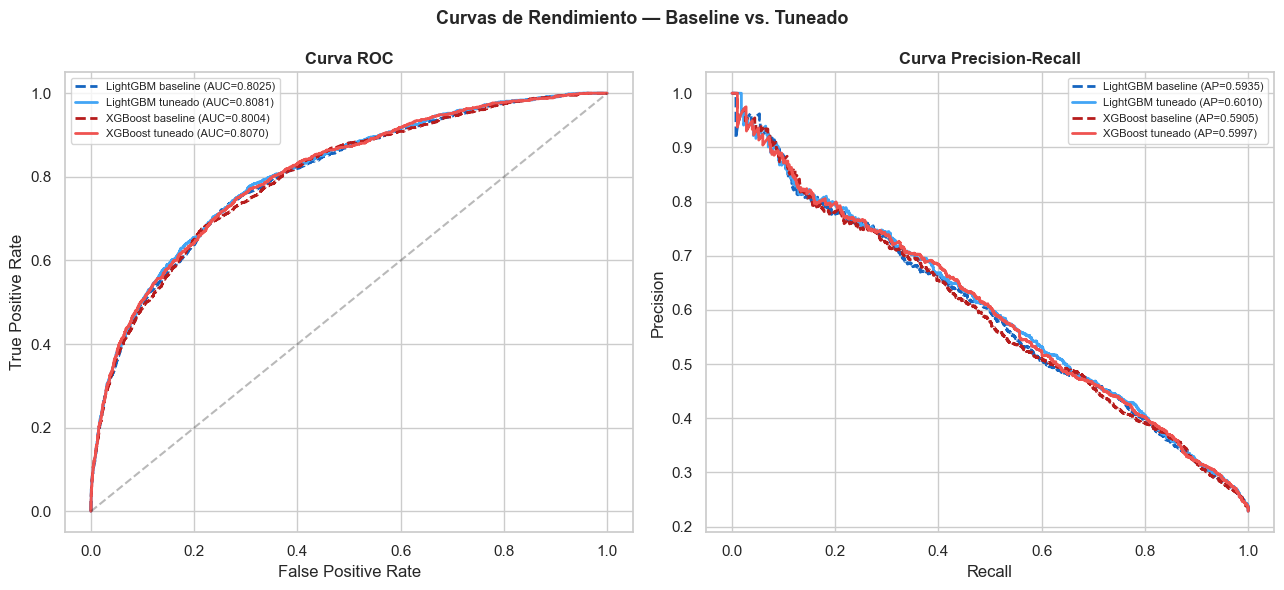
\includegraphics[width=\columnwidth]{fig_feature_importance.png}
  \caption{Top 20 variables por importancia de ganancia para LightGBM (izquierda) y XGBoost (derecha) en sus versiones tuneadas. Ambos modelos coinciden en las variables líderes (\texttt{top\_category}, \texttt{recency\_days}), validando la consistencia del análisis.}
  \label{fig:fi}
\end{figure}

% ──────────────────────────────────────────────────────────────────
\section{Serialización y Verificación de Reproducibilidad}

\subsection{Pipeline de Producción}
El modelo final se exporta como un \texttt{Pipeline} de scikit-learn que encapsula el preprocesador y el clasificador en un único artefacto:

\begin{equation}
\texttt{pipeline} = [\text{ColumnTransformer} \to \text{LGBMClassifier}(\boldsymbol{\theta}^*)]
\end{equation}

Este diseño garantiza que en producción se aplique exactamente el mismo preprocesamiento utilizado en entrenamiento, eliminando el riesgo de inconsistencias por transformaciones omitidas o aplicadas en distinto orden.

\subsection{Verificación Round-Trip}
El notebook \texttt{04\_evaluacion\_modelo\_final.ipynb} reconstruye el pipeline desde \texttt{10\_tuning\_results.json}, lo entrena sobre el conjunto de desarrollo y verifica que el modelo serializado (\texttt{modelo\_final.pkl}) produce predicciones idénticas al pipeline en memoria, con una diferencia en ROC-AUC inferior a $10^{-8}$.

\subsection{Comparación con Sprints Anteriores}
La Tabla~\ref{tab:evolution} resume la evolución del rendimiento a lo largo de los tres sprints.

\begin{table}[h]
\centering
\caption{Evolución de Métricas por Sprint}
\label{tab:evolution}
\resizebox{\columnwidth}{!}{%
\begin{tabular}{lrrrr}
\toprule
Sprint & Modelo & ROC-AUC & Recall & F1 \\
\midrule
S1 (baseline) & Logística (RFMT básico) & 0.5355 & 0.16 & 0.21 \\
S2 (pipeline) & Random Forest, 28 feat. & 0.7929 & 0.63 & 0.54 \\
\textbf{S3 (final)} & \textbf{LightGBM tuneado} & \textbf{0.8081} & \textbf{0.66} & \textbf{0.56} \\
\midrule
Mejora S1 $\to$ S3 & & +50.8\% & +312.5\% & +166.7\% \\
Mejora S2 $\to$ S3 & & +1.9\%  & +4.9\%   & +3.7\% \\
\bottomrule
\end{tabular}%
}
\end{table}

% ──────────────────────────────────────────────────────────────────
\section{Conclusiones y Próximos Pasos}

\subsection{Conclusiones}
El Sprint 3 entregó los siguientes resultados verificables:

\begin{enumerate}
    \item \textbf{Benchmark comparativo} de cinco modelos sobre el set oficial de 28 features y split temporal del Sprint 2, con métricas completas (ROC-AUC, Gini, PR-AUC, F1, Precision, Recall, gap de sobreajuste).
    \item \textbf{Selección justificada} de LightGBM y XGBoost como finalistas mediante ranking compuesto, evitando la trampa de ordenar únicamente por ROC-AUC que habría seleccionado a Gradient Boosting con Recall inaceptable (0.33).
    \item \textbf{HPO con Optuna TPE} (50 \textit{trials} por modelo): LightGBM mejoró +0.0046 en ROC-AUC; XGBoost mejoró +0.0088 en ROC-AUC pero redujo su Recall en 4 puntos al optimizar para AUC.
    \item \textbf{Modelo final} LightGBM tuneado: ROC-AUC = 0.8081, Gini = 0.6162, Recall = 0.6617 (umbral 0.50), con umbral óptimo F1 en 0.55.
    \item \textbf{Interpretabilidad}: \texttt{top\_category} y \texttt{recency\_days} explican el 43\% de la ganancia del modelo, confirmando que el tipo de producto y la temporalidad de la compra son los mejores discriminadores del segmento premium en el contexto de la Paradoja del Target.
    \item \textbf{Artefacto serializado} (\texttt{modelo\_final.pkl}): pipeline reproducible verificado con delta ROC-AUC $< 10^{-8}$ en la verificación round-trip.
\end{enumerate}

\subsection{Próximos Pasos — Sprint 4}
Para el Sprint 4 se propone:
\begin{enumerate}
    \item \textbf{API de scoring (FastAPI):} Endpoint REST que recibe las 28 features de un cliente y retorna \texttt{is\_premium} con la probabilidad asociada, usando \texttt{modelo\_final.pkl}.
    \item \textbf{Dashboard (Streamlit):} Visualización del segmento premium identificado, KPIs de negocio actualizados y distribución de scores por estado geográfico.
    \item \textbf{Gobernanza y ética:} Análisis de equidad del clasificador por \texttt{customer\_state} y \texttt{region\_group} (las variables geográficas tienen 6.4\% de importancia combinada), para detectar posibles sesgos de cobertura por región.
    \item \textbf{Reentrenamiento mensual:} Script orquestador que ejecuta el pipeline completo —desde la master table hasta la exportación de un nuevo \texttt{.pkl}— sobre datos actualizados, manteniendo el umbral P80 en modo \texttt{apply}.
    \item \textbf{HPO orientado a Recall:} Explorar una corrida adicional de Optuna con Recall como función objetivo para XGBoost, dado el trade-off observado en este sprint.
\end{enumerate}

\begin{thebibliography}{1}

\bibitem{sprint1_report}
M. de la Quintana, G. Nina, y G. Toro,
``Reporte de Sprint 1: Perfilado de Datos Crudos, Exploración y Modelo Baseline para la Identificación de Clientes Premium,''
\textit{Informe Técnico, Módulo de Implementación de Soluciones de IA, Maestría en IA y Ciencia de Datos}, mayo 2026.

\bibitem{sprint2_report}
M. de la Quintana, G. Nina, y G. Toro,
``Reporte de Sprint 2: Pipeline Reproducible de Ingeniería de Variables y Clasificación de Clientes Premium,''
\textit{Informe Técnico, Módulo de Implementación de Soluciones de IA, Maestría en IA y Ciencia de Datos}, junio 2026.

\bibitem{rfmt_methodology}
A. Ullah, M. I. Mohmand, H. Hussain, S. Johar, I. Khan, S. Ahmad, H. A. Mahmoud, and S. Huda,
``Customer Analysis Using Machine Learning-Based Classification Algorithms for Effective Segmentation Using Recency, Frequency, Monetary, and Time,''
\emph{Sensors}, vol. 23, no. 6, p. 3180, Mar. 2023. [Online]. Available: \url{https://doi.org/10.3390/s23063180}

\bibitem{optuna2019}
T. Akiba, S. Sano, T. Yanase, T. Ohta, and M. Koyama,
``Optuna: A Next-generation Hyperparameter Optimization Framework,''
in \textit{Proc. ACM KDD}, 2019. [Online]. Available: \url{https://doi.org/10.1145/3292500.3330701}

\bibitem{bergstra2011}
J. Bergstra, R. Bardenet, Y. Bengio, and B. Kégl,
``Algorithms for Hyper-Parameter Optimization,''
in \textit{Advances in Neural Information Processing Systems (NeurIPS)}, vol. 24, 2011.

\bibitem{lightgbm2017}
G. Ke, Q. Meng, T. Finley, T. Wang, W. Chen, W. Ma, Q. Ye, and T.-Y. Liu,
``LightGBM: A Highly Efficient Gradient Boosting Decision Tree,''
in \textit{Advances in Neural Information Processing Systems (NeurIPS)}, vol. 30, 2017.

\bibitem{xgboost2016}
T. Chen and C. Guestrin,
``XGBoost: A Scalable Tree Boosting System,''
in \textit{Proc. ACM KDD}, pp. 785--794, 2016. [Online]. Available: \url{https://doi.org/10.1145/2939672.2939785}

\end{thebibliography}

\end{document}
